\documentclass[Master,english,Harvard]{twbook}
\usepackage[utf8]{inputenc}
\usepackage[T1]{fontenc}
\usepackage{csquotes}
\usepackage{graphicx}
\usepackage{amsmath}
\usepackage{booktabs}
\usepackage{hyperref}
\usepackage{acronym} % geladen von twbook.cls; nohyperlinks via \PassOptionsToPackage in mt_bhinder.tex
\usepackage[most]{tcolorbox}
\usepackage{listings}
\usepackage{float} % erlaubt [H] fuer harte Float-Platzierung
\usepackage{longtable} % seitenumbrechende Tabellen
\usepackage{pdflscape} % echte Querformat-Seiten (PDF-Viewer zeigt horizontal)
% Absatzstil: kein Erstzeilen-Einzug, stattdessen vertikaler Abstand
% zwischen Absaetzen (Blockstil wie in der Salma-Arbeit).
\usepackage{parskip}

% Bibliografie: kein haengender Einzug in den Folgezeilen, dafuer
% kleiner Abstand zwischen den Eintraegen.
\setlength{\bibhang}{0pt}
\setlength{\bibitemsep}{0.6\baselineskip}

% Sentence Case auch fuer die generierten Verzeichnis-Titel
% (Konsistenz mit den Kapitel-/Section-Ueberschriften).
\addto\captionsenglish{%
    \renewcommand*{\listfigurename}{List of figures}%
    \renewcommand*{\listtablename}{List of tables}%
}
\renewcommand*{\listacroname}{List of abbreviations}
\graphicspath{{images/}}

% Stil fuer Prompt-/Code-Listings (z.B. lst:system-prompt in Kap. 3.5)
\lstset{
    basicstyle=\ttfamily\small,
    breaklines=true,
    frame=single,
    framerule=0.5pt,
    xleftmargin=2mm,
    captionpos=b}

% Box fuer Forschungsfragen (Kap. 1) und deren Beantwortung (Kap. 4).
% Schlichter Rahmen: duenne graue Linie, weisser Koerper, hellgraue
% Titelzeile, eckige Kanten.
% Box fuer Antwort-Auszuege in Kap. 4 (gleiche Optik wie rqbox).
\newtcolorbox{responsebox}[1]{%
    breakable,
    sharp corners,
    colback=gray!2,
    colframe=black!60,
    colbacktitle=black!8,
    coltitle=black,
    fonttitle=\bfseries\small,
    fontupper=\small,
    title={#1},
    boxrule=0.5pt,
    left=2mm, right=2mm, top=1.5mm, bottom=1.5mm}

\newtcolorbox{rqbox}[1]{%
    breakable,
    sharp corners,
    colback=white,
    colframe=black!60,
    colbacktitle=black!8,
    coltitle=black,
    fonttitle=\bfseries,
    title={#1},
    boxrule=0.5pt,
    left=2mm, right=2mm, top=1.5mm, bottom=1.5mm}

\title{Retrieval-Augmented Generation for Cyber Threat Intelligence: Designing and Evaluating a Prototype to Support Security Analysts}
\author{Joben Preet Bhinder, BSc.}
\studentnumber{2410302067}
\supervisor{Wolfgang Rogner, BSc. MSc.}
\secondsupervisor{Tamás Horváth, BSc. MSc.}
\place{Vienna}
\degreecourse{Information Systems Management}

\addbibresource{references.bib}

\kurzfassung{% Spiegelpaar zu content/frontmatter/abstract.tex — inhaltlich identisch
% halten (destilliert aus Kap. 5.1 und den RQ-Boxen in 4.7).
Cyber Threat Intelligence (CTI) verlangt von Analysten, Bedrohungs\-informationen
aus heterogenen Quellen unter Zeitdruck zu korrelieren. Large Language
Models (LLMs) k\"onnen diese Arbeit unterst\"utzen, scheitern im direkten
Einsatz jedoch an drei Grenzen: veraltetem Modellwissen, Halluzinationen
und fehlender Provenienz der Aussagen.

Diese Masterarbeit untersucht, wie Retrieval-Augmented Generation (RAG)
die Qualit\"at, Verl\"asslichkeit und operative N\"utzlichkeit von
CTI-Analyse und Threat-Hunting-Workflows verbessern kann. Dazu wird ein
Open-Source-Prototyp konzipiert, implementiert und evaluiert, der vier
kuratierte CTI-Quellen (NVD, CISA KEV, CISA-Advisories, MISP; 84.982
Dokumente) in einen provenienz-erhaltenden Index \"uberf\"uhrt. Ein
hybrides Retrieval kombiniert BM25 und dichte Vektorsuche mit
Cross-Encoder-Reranking. Die Antwortgenerierung ist geschichtet:
Verifizierbare Fakten werden deterministisch aus Passagen-Metadaten
gerendert, ein lokal betriebenes 8B-Modell liefert ausschlie\ss lich das
Narrativ, mit erzwungenen, validierten Zitaten und expliziter
Enthaltung ohne Evidenz.

Die Evaluation vergleicht sechs Konfigurationen -- von der
retrieval-freien Baseline bis zur gehosteten Ablation -- auf einem
eingefrorenen Index-Stand mit 28 Queries \"uber vier
Analyst-Task-Typen und drei L\"aufen je Konfiguration. Bewertet wird
mit RAGAS, Field Coverage und einem vierdimensionalen
Analysten-Rubric samt szenariobasierter Analyse. Zentrales Ergebnis:
Die Antwortkorrektheit bleibt auf Baseline-Niveau, die
Nachvollziehbarkeit (Traceability) steigt jedoch von 1,23 auf 2,56 --
Retrieval liefert auf diesem Query-Set in erster Linie
Verifizierbarkeit, nicht h\"ohere Korrektheit.

Der wissenschaftliche Beitrag umfasst Workflow-\"ubergreifende
empirische Evidenz f\"ur RAG in der CTI, den Befund, dass generische
RAG-Metriken und analystenorientierte Ma\ss e auseinanderfallen, sowie
ein Referenzmodell mit acht empirisch begr\"undeten Designprinzipien.
Der praktische Beitrag ist ein reproduzierbares, lokal betreibbares
System samt quantifiziertem Local-versus-Hosted-Trade-off.
}
\schlagworte{RAG, Cyber Threat Intelligence, Retrieval-Augmented Generation, Evaluation}

\outline{% Mirror of content/frontmatter/kurzfassung.tex — keep the content
% identical (distilled from Section 5.1 and the RQ boxes in 4.7).
Cyber Threat Intelligence (CTI) requires analysts to correlate threat
information from heterogeneous sources under time pressure. Large
Language Models (LLMs) can support this work but face three limits in
direct use: outdated parametric knowledge, hallucination, and missing
provenance.

This master's thesis examines how Retrieval-Augmented Generation (RAG)
can improve the quality, reliability, and operational usefulness of
CTI analysis and threat-hunting workflows. An open-source prototype is
designed, implemented, and evaluated that ingests four curated CTI
sources (NVD, CISA KEV, CISA advisories, MISP; 84,982 documents) into
a provenance-preserving index. Hybrid retrieval combines BM25 and
dense vector search with cross-encoder reranking. Answer generation is
layered: verifiable facts are rendered deterministically from passage
metadata, and a locally deployed 8B model contributes only the
narrative, with enforced, validated citations and explicit abstention
without evidence.

The evaluation compares six configurations, from a non-retrieval
baseline to a hosted ablation, on a frozen index state with 28 queries
across four analyst task types and three runs per configuration,
scored with RAGAS, field coverage, and a four-dimension analyst rubric
complemented by scenario analysis. The central finding is that answer
correctness stays at baseline level while traceability rises from 1.23
to 2.56: on this query set, retrieval buys verifiability rather than
raw correctness.

The scientific contribution comprises workflow-level empirical
evidence for RAG in CTI, the finding that generic RAG metrics and
analyst-oriented measures diverge, and a reference model with eight
empirically grounded design principles. The practical contribution is
a reproducible, locally deployable system together with a quantified
local-versus-hosted trade-off.
}
\keywords{RAG, Cyber Threat Intelligence, Retrieval-Augmented Generation, Evaluation}
\acknowledgements{I would like to thank everyone who accompanied me during the writing
of this thesis.

My particular thanks go to my supervisor, Wolfgang Rogner, for his
guidance, his clear and constructive feedback, and for the discussions
that sharpened this work from the first proposal draft to the final
chapters. I also thank Tam\'as Horv\'ath for co-supervising this
thesis.

My heartfelt thanks go to my family, whose support, patience, and
encouragement carried me through this thesis and the years of study
that led to it. Without them, this work would not have been possible.
}

\begin{document}

\maketitle

\chapter{Introduction}

\section{Problem statement and motivation}
...

\section{State of the art}
...

\section{Research questions and objectives}
...
% ======================================================================
% Kapitel 2 — Background and Related Work (Budget: ~2,5 Seiten, KURZ)
% Struktur nach Salmas Kapitel 2 (Erkenntnisse + Luecken), plus eine
% kompakte Foundations-Section, weil CTI-/RAG-Begriffe nicht
% selbsterklaerend sind. Keine Designkriterien, keine Evaluations-
% methodik hier --- das lebt in Kap. 3 (\ref{sec:requirements}, \ref{sec:evaluation-design}).
% ======================================================================
\chapter{Background and Related Work}
\label{ch:background}

\section{CTI and RAG foundations}
\label{sec:cti}
% B1--B3 speisen die Gaps (\ref{sec:research-gap}) und Kriterien
% (\ref{sec:requirements}); Rueckverweis in \ref{sec:assessment}.

Cyber Threat Intelligence (CTI) is evidence-based knowledge about existing
or emerging threats, including context, indicators, and actionable advice
that informs security decisions \parencite{sun2023ctimining}. In practice,
CTI is communicated through recurring artifact types. Indicators of
Compromise (IOCs) are forensic artifacts, such as file hashes, IP
addresses, or domains, that indicate a compromised system
\parencite{palacin2021threat}. Tactics, Techniques, and Procedures (TTPs)
describe adversary behavior on three levels: the tactical goal, the method
used to achieve it, and its concrete implementation
\parencite{ismail2025wazuh}. The MITRE ATT\&CK framework is the industry
standard for categorizing these behaviors \parencite{lekssays2025techniquerag}.
Threat hunting builds on CTI: analysts proactively and iteratively search
their environment for signs of compromise that automated detection has
missed, typically starting from intelligence about the adversary
\parencite{palacin2021threat,sun2023ctimining}.

Analyst workflows follow a recurring cycle from planning and collection
through processing and analysis to dissemination
\parencite{palacin2021threat}. Across this cycle, the literature reports
three bottlenecks:
% TODO: sobald die Workflow-Abbildung vorliegt, hier einen Verweissatz
% auf Figure~\ref{fig:analyst-workflow} ergaenzen.

% TODO Abbildung: generischer CTI-Analyst-Workflow (Feed-/Report-Eingang
% -> Triage -> Anreicherung/Korrelation -> Bewertung/Report), mit
% markierten Engpaessen B1--B3. Als drawio anlegen (docs/architecture/).
% \begin{figure}[htbp]
%     \centering
%     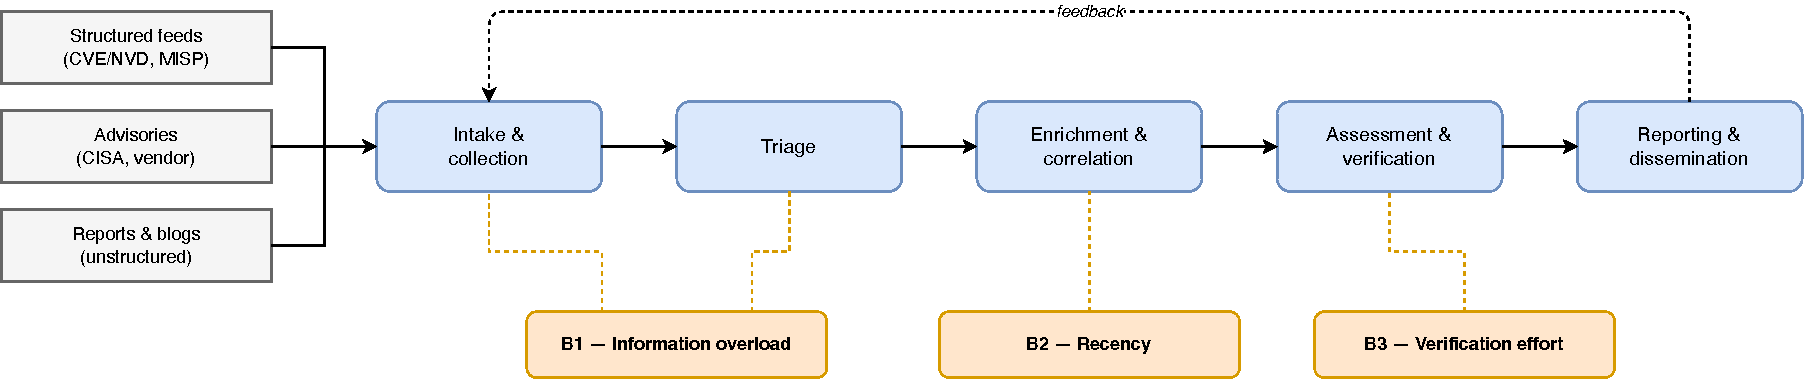
\includegraphics[width=0.9\textwidth]{cti_analyst_workflow}
%     \caption{Generic CTI analyst workflow with bottlenecks B1--B3}
%     \label{fig:analyst-workflow}
% \end{figure}

\begin{enumerate}
    \item \textbf{B1 --- Information overload:} the volume, heterogeneity,
          and informal structure of threat feeds and reports exceed what
          analysts can process consistently
          \parencite{alhuzali2025llm,rastogi2023soc}.
    \item \textbf{B2 --- Recency:} threat knowledge changes faster than
          static knowledge bases, including the parametric knowledge of
          trained language models, can follow
          \parencite{paul2025proactive,chen2023benchmarking}.
    \item \textbf{B3 --- Verification effort:} extracting information from
          unstructured reports and validating it remains manual expert
          work, and outputs without transparent provenance cannot be acted
          on \parencite{rajapaksha2024rag,tseng2024llm}.
\end{enumerate}

Retrieval-Augmented Generation (RAG) grounds LLM output in external
knowledge. A RAG pipeline indexes documents by cleaning, chunking, and
embedding them, retrieves the passages most relevant to a query, optionally
reranks them, and assembles them into the prompt from which the model
generates its answer \parencite{gao2024rag}. This design targets the LLM
limitations most relevant to CTI: hallucination, outdated knowledge, and
reasoning that cannot be traced to sources
\parencite{gao2024rag,chen2023benchmarking}.
% TODO: sobald die Pipeline-Abbildung vorliegt, Verweissatz auf
% Figure~\ref{fig:rag-pipeline} ergaenzen.

Retrieval can be sparse, dense, or hybrid;
Table~\ref{tab:retrieval-strategies} contrasts the strategies and the role
of reranking \parencite{agnihotram2025retrieval}.

\begin{table}[H]
    \centering
    \small
    \begin{tabular}{lp{0.26\textwidth}p{0.24\textwidth}p{0.24\textwidth}}
        \toprule
        \textbf{Strategy} & \textbf{Principle} & \textbf{Strength} & \textbf{Limitation} \\
        \midrule
        Sparse (BM25) & exact term matching with term-frequency weighting
            & efficient; reliable for explicit identifiers
            & misses semantically equivalent formulations \\
        Dense & embeddings in a shared vector space
            & captures paraphrases and related concepts
            & can surface related yet irrelevant passages \\
        Hybrid & parallel sparse and dense retrieval, merged by rank or
                 score fusion
            & keeps exact matches while adding semantic coverage
            & merged list still needs reordering \\
        Reranking & cross-encoder scores each query--passage pair
            & raises precision with little recall loss
            & adds latency \\
        \bottomrule
    \end{tabular}
    \caption{Retrieval strategies and reranking in RAG pipelines}
    \label{tab:retrieval-strategies}
\end{table}

These trade-offs matter for CTI text, where the same threat actor appears
under aliases such as APT28 and Fancy Bear and distinct ATT\&CK techniques
share overlapping keywords; hybrid retrieval with reranking therefore
suits CTI corpora \parencite{alhuzali2025llm,lekssays2025techniquerag}.
Citing the retrieved sources in the generated answer makes it verifiable:
analysts can inspect the evidence behind each claim instead of trusting
the model \parencite{rajapaksha2024rag,liu2023trustworthy}.

% TODO Abbildung: generische RAG-Pipeline (Ingestion -> Chunking ->
% Indexing -> Retrieval -> Reranking -> Context Assembly -> Generation).
% Ersetzt Prosa-Definitionen; 3.2 zeigt spaeter die konkrete Instanz.
% \begin{figure}[htbp]
%     \centering
%     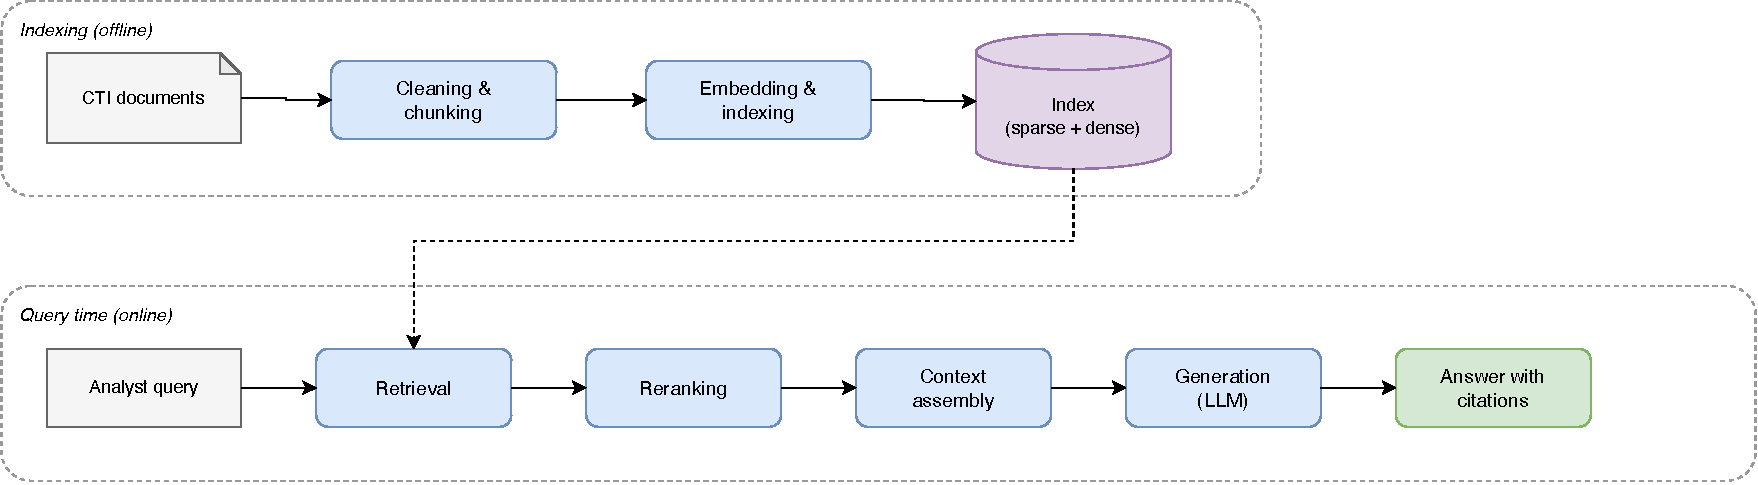
\includegraphics[width=\textwidth]{rag_pipeline_generic}
%     \caption{Generic RAG pipeline stages}
%     \label{fig:rag-pipeline}
% \end{figure}

\section{Key findings from the literature}
\label{sec:literature-findings}

The literature review covers four topic areas: CTI analyst workflows, LLMs
in cybersecurity, RAG for CTI, and the evaluation of RAG systems.
Table~\ref{tab:literature-findings} summarizes the key findings; the
research gaps in Section~\ref{sec:research-gap} follow from them.

\begingroup
\small
\begin{longtable}{p{0.15\textwidth}p{0.53\textwidth}p{0.22\textwidth}}
        \toprule
        \textbf{Topic area} & \textbf{Key finding} & \textbf{Source} \\
        \midrule
        \endfirsthead
        \toprule
        \textbf{Topic area} & \textbf{Key finding} & \textbf{Source} \\
        \midrule
        \endhead
        \midrule
        \multicolumn{3}{r@{}}{\footnotesize\itshape continued on next page} \\
        \endfoot
        \bottomrule
        \caption{Key findings of the literature review}
        \label{tab:literature-findings}
        \endlastfoot
        CTI analyst workflows
        & The volume and the non-uniform, informal structure of threat
          feeds overwhelm analysts; fully automated processing is not
          feasible & \cite{rastogi2023soc,alhuzali2025llm} \\
        & Analyzing natural-language CTI reports is labor-intensive and
          repetitive and delays response
          & \cite{tseng2024llm,rajapaksha2024rag} \\
        \midrule
        LLMs in cybersecurity
        & LLMs support vulnerability analysis, report summarization, and
          IOC/TTP extraction; junior analysts gain the most
          & \cite{divakaran2024llm} \\
        & Recurring failure modes are hallucination, outdated knowledge,
          and technical misinterpretation & \cite{alhuzali2025llm} \\
        & LLMs over-trust retrieved context and can be misled by incorrect
          information in it & \cite{chen2023benchmarking} \\
        \midrule
        RAG for CTI
        & Hybrid retrieval with reranking addresses terminology variance
          (actor aliases) and overlapping keywords in security text
          & \cite{alhuzali2025llm,lekssays2025techniquerag} \\
        & Retrieval grounding raises precision in TTP mapping, where
          decoder-only LLMs show high recall but low precision
          & \cite{fayyazi2024ttp} \\
        & Existing CTI-RAG prototypes each target a single task, e.g.\
          attack investigation, technique annotation, event response, or
          IOC extraction
          & \cite{alhuzali2025llm,lekssays2025techniquerag,ismail2025wazuh,tseng2024llm} \\
        \midrule
        RAG evaluation
        & Retrieval is assessed with Precision@k and Recall@k plus
          rank-aware metrics such as MRR and nDCG
          & \cite{agnihotram2025retrieval,yu2024evaluation} \\
        & Reference-free frameworks (RAGAS, ARES) score faithfulness,
          answer relevancy, and context relevance without gold answers
          & \cite{es2023ragas,saadfalcon2024ares} \\
        & LLM-as-a-judge scoring risks reinforcing model biases and can
          diverge from human judgment in specialized domains
          & \cite{akkiraju2024facts,yu2024evaluation} \\
        & Industrial ground-truth datasets for CTI tasks are scarce; only
          few public benchmarks (e.g.\ CTIBench) exist
          & \cite{xu2025llm,alhuzali2025llm} \\
\end{longtable}
\endgroup

\section{Research gaps}
\label{sec:research-gap}

From the findings in Table~\ref{tab:literature-findings}, three research
gaps are derived:

\begin{enumerate}
    \item \textbf{G1 --- Workflow-level empirical evidence:} Existing
          CTI-RAG prototypes each address a single task, such as attack
          investigation or technique annotation. How RAG performs across
          the range of tasks an analyst works through, and which
          architectural choices drive that performance, remains
          empirically open.
    \item \textbf{G2 --- Evaluation realism:} Reported evaluations center
          on controlled benchmarks and isolated technical metrics, and
          ground-truth datasets for CTI tasks are scarce. Evidence that
          connects retrieval and generation quality to representative
          analyst tasks is rare.
    \item \textbf{G3 --- Source reliability:} RAG pipelines can ingest and
          propagate misinformation, and LLMs tend to over-trust retrieved
          context. How CTI-RAG systems should account for the integrity
          and reliability of their sources is not settled.
\end{enumerate}

These gaps, together with the workflow bottlenecks B1--B3 from
Section~\ref{sec:cti}, define the design space of this thesis:
Section~\ref{sec:requirements} derives design criteria from them, and
Section~\ref{sec:assessment} assesses the prototype against these
criteria.

% ======================================================================
% Kapitel 3 — Solution: Design and Implementation (Budget: ~9 Seiten)
% Einzige Heimat fuer: Designkriterien (3.2) und Evaluationsdesign (3.8).
% Architektur begruendet nichts neu, sondern referenziert Kriterien-IDs.
% ======================================================================
\chapter{Solution: Design and Implementation}
\label{ch:solution}

\section{Task formulation}
\label{sec:task-formulation}

The task addressed in this thesis is grounded question answering over CTI
sources. The prototype operates on a corpus $\mathcal{D}$ of documents
collected from heterogeneous CTI sources and segmented into a set of
passages $\mathcal{P}$ (Section~\ref{sec:ingestion}). Given an analyst
query $q$, a retrieval function $R$ selects the $k$ highest-ranked passages
as context:
\begin{equation}
    \mathcal{C}_k = R(q, \mathcal{P}), \qquad \lvert\mathcal{C}_k\rvert = k.
    \label{eq:retrieval}
\end{equation}
A generation model $g$ then produces the answer
\begin{equation}
    a = g(q, \mathcal{C}_k),
    \label{eq:generation}
\end{equation}
subject to a grounding constraint: every factual claim in $a$ must be
attributable to at least one passage in $\mathcal{C}_k$ and marked with an
inline citation to that passage. The analyst can therefore verify each
claim against its source instead of trusting the answer as a whole
(bottleneck B3, Section~\ref{sec:cti}).

In the hybrid configuration, $R$ combines a lexical relevance score
(BM25) with a semantic similarity score (dense embeddings) and reranks the
fused candidates; Section~\ref{sec:retrieval} describes this instantiation.
Setting $\mathcal{C}_k = \emptyset$ yields the non-retrieval baseline
\begin{equation}
    a_0 = g(q, \emptyset),
    \label{eq:baseline}
\end{equation}
in which the model answers from parametric knowledge alone. This baseline
corresponds to configuration V0 in the evaluation
(Section~\ref{sec:baselines}); the comparison between $a$ and $a_0$
quantifies the effect of retrieval augmentation and thereby
operationalizes SRQ1.

\section{Requirements and design criteria}
\label{sec:requirements}
% TODO: EINZIGE Stelle fuer Designkriterien. Aus Forschungsluecken
% (\ref{sec:research-gap}) UND Workflow-Engpaessen B1--B3 (\ref{sec:cti})
% ableiten --- im Einleitungstext der Section beide Quellen explizit nennen.
% Rueckverfolgbarkeitskette: B/G -> Criterion -> Result -> RQ-Antwort.
% Zuordnung (fuer Herleitungstext): C1 <- B3/G1, C2 <- B1/G1, C3 <- G3,
% C4 <- G2, C5 <- B1/G2, C6 <- Proposal-Vorgabe (open-source only).

% Kriterien-Entwuerfe direkt aus SotA Kap. 4.2 "Implications for this
% thesis" + Proposal (open-source only). Beim Schreiben: pro Kriterium
% 1--2 Saetze Herleitung mit Gap-Bezug (G1--G3), dann nur noch per ID
% referenzieren.
\begin{table}[htbp]
    \centering
    \small
    \begin{tabular}{lp{0.62\textwidth}ll}
        \toprule
        \textbf{ID} & \textbf{Design criterion} & \textbf{Gap} & \textbf{Ref.} \\
        \midrule
        C1 & Evidence-linked outputs: explicit, source-based citations for
             key claims to support traceability and reduce verification
             effort & G1 & SRQ1 \\
        C2 & Hybrid retrieval as a baseline: combined lexical (BM25) and
             semantic retrieval with optional reranking & G1 & SRQ1 \\
        C3 & Source integrity and reliability: curated ingestion and
             source-reliability signals to limit misinformation risk & G3 & MRQ \\
        C4 & Scenario-based evaluation: assessment on representative CTI
             analyst tasks beyond offline metrics & G2 & SRQ2 \\
        C5 & Analyst-oriented presentation: structured outputs matching
             analyst intent (task coverage, clarity, transparency) & G2 & SRQ2 \\
        C6 & Open-source, locally deployable stack (data protection,
             reproducibility, cost) & --- & MRQ \\
        \bottomrule
    \end{tabular}
    \caption{Design criteria with traceability to research gaps and research questions}
    \label{tab:design-criteria}
\end{table}

\section{System architecture}
\label{sec:architecture}
% TODO: Komponenten und Datenfluss beschreiben. Designentscheidungen NUR
% per Kriterien-ID begruenden ("addresses C2"), keine erneute Herleitung.
...

% TODO Abbildung: Export aus docs/architecture/cti_rag_architecture_overview.drawio
% -> images/ (PDF/PNG). Konkrete Instanz von \ref{fig:rag-pipeline}.
% \begin{figure}[htbp]
%     \centering
%     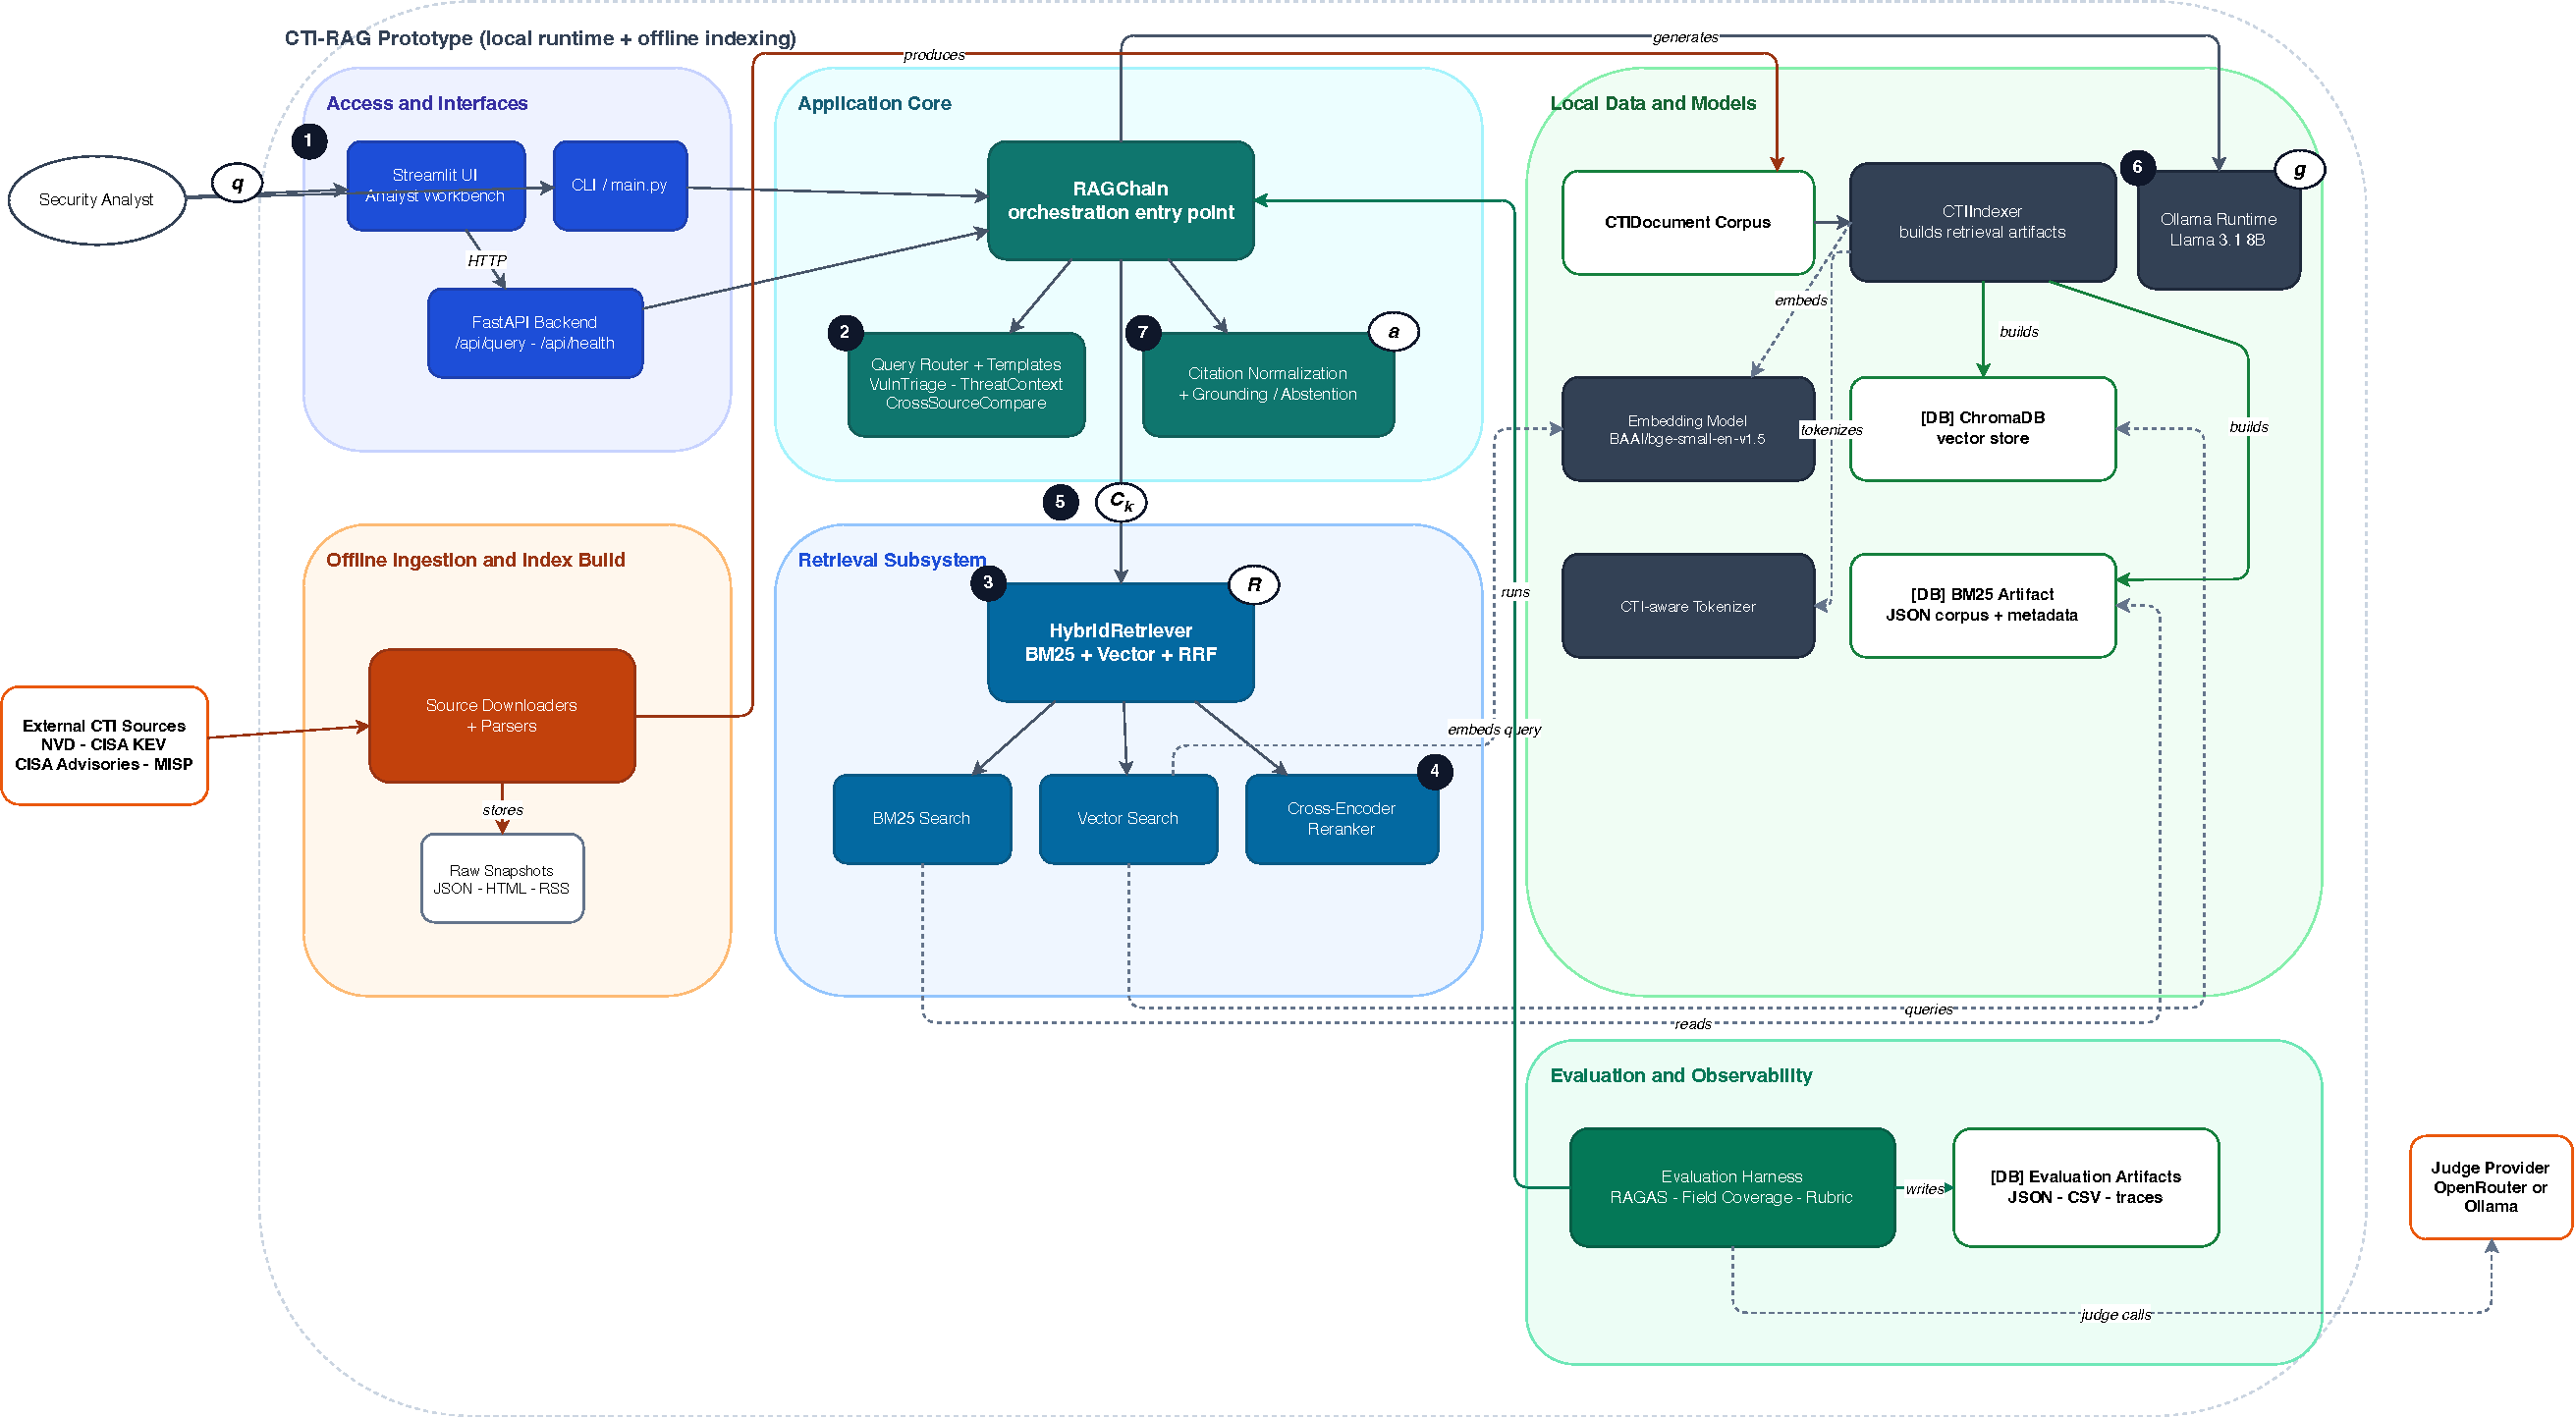
\includegraphics[width=\textwidth]{cti_rag_architecture_overview}
%     \caption{System architecture of the CTI-RAG prototype}
%     \label{fig:architecture}
% \end{figure}

\section{Data ingestion and preprocessing}
\label{sec:ingestion}
% TODO: Quellenkorpus (welche CTI-Quellen, Umfang), Parsing, Chunking,
% Metadaten.
...

% TODO Tabelle: Korpus-Statistik aus dem Index ziehen.
% \begin{table}[htbp]
%     \centering\small
%     \begin{tabular}{llrr}
%         \toprule
%         \textbf{Source} & \textbf{Document type} & \textbf{Documents} & \textbf{Chunks} \\
%         \midrule
%         CVE/NVD & ... & ... & ... \\
%         CISA advisories & ... & ... & ... \\
%         MISP & ... & ... & ... \\
%         Vendor reports & ... & ... & ... \\
%         \bottomrule
%     \end{tabular}
%     \caption{Corpus statistics of the ingested CTI sources}
%     \label{tab:corpus-stats}
% \end{table}

\section{Hybrid retrieval and reranking}
\label{sec:retrieval}
% TODO: dense + BM25, Fusion, Reranker. Kein eigenes Diagramm ---
% der Fluss steckt in \ref{fig:architecture}.
...

% TODO Tabelle: Werte aus configs/settings.yaml uebernehmen.
% \begin{table}[htbp]
%     \centering\small
%     \begin{tabular}{llp{0.42\textwidth}}
%         \toprule
%         \textbf{Component} & \textbf{Model / method} & \textbf{Parameters} \\
%         \midrule
%         Sparse retrieval & BM25 & ... \\
%         Dense retrieval & <embedding model> & ... \\
%         Fusion & ... & ... \\
%         Reranking & <cross-encoder> & top-k = ... \\
%         \bottomrule
%     \end{tabular}
%     \caption{Retrieval pipeline configuration}
%     \label{tab:retrieval-config}
% \end{table}

\section{Context assembly, answer generation and citation}
\label{sec:generation}
% TODO: Kontextaufbau, Prompt-Struktur (Verweis auf Anhang Prompt Templates),
% Grounding-/Zitiermechanismus, Refusal-Verhalten bei fehlender Evidenz.
...

% TODO Listing: gekuerztes System-Prompt mit Zitier-Instruktion
% (aus src/cti_rag/rag/prompts.py); Vollversion in Anhang B.
% \begin{lstlisting}[caption={System prompt with citation instruction (excerpt)},
%                    label={lst:system-prompt}]
% ...
% \end{lstlisting}

\section{Implementation}
\label{sec:implementation}
% TODO: Technologie-Stack, Verweis auf Repository (Anhang).
% Hinweis: MCP-/Agent-Erweiterung hier nur kurz erwaehnen oder ganz in
% Future Work (\ref{sec:future-work}) verschieben.
...

% TODO Tabelle: Komponenten nach Salmas Vorbild (ihre Tabelle 11).
% \begin{table}[htbp]
%     \centering\small
%     \begin{tabular}{lp{0.22\textwidth}p{0.45\textwidth}}
%         \toprule
%         \textbf{Path} & \textbf{Function} & \textbf{Details} \\
%         \midrule
%         src/cti\_rag/ingestion/ & ... & ... \\
%         src/cti\_rag/retrieval/ & Hybrid retrieval & ... \\
%         src/cti\_rag/rag/ & Chain, prompts & ... \\
%         src/cti\_rag/evaluation/ & RAGAS evaluation & ... \\
%         \bottomrule
%     \end{tabular}
%     \caption{Prototype components with path, function, and technical details}
%     \label{tab:components}
% \end{table}

% TODO Abbildung: UI-Screenshot (Chat-Ansicht mit Pipeline-Flow-Card oder
% Landing Page). Druckbarkeit des Dark-Themes pruefen, ggf. helles Theme.
% \begin{figure}[htbp]
%     \centering
%     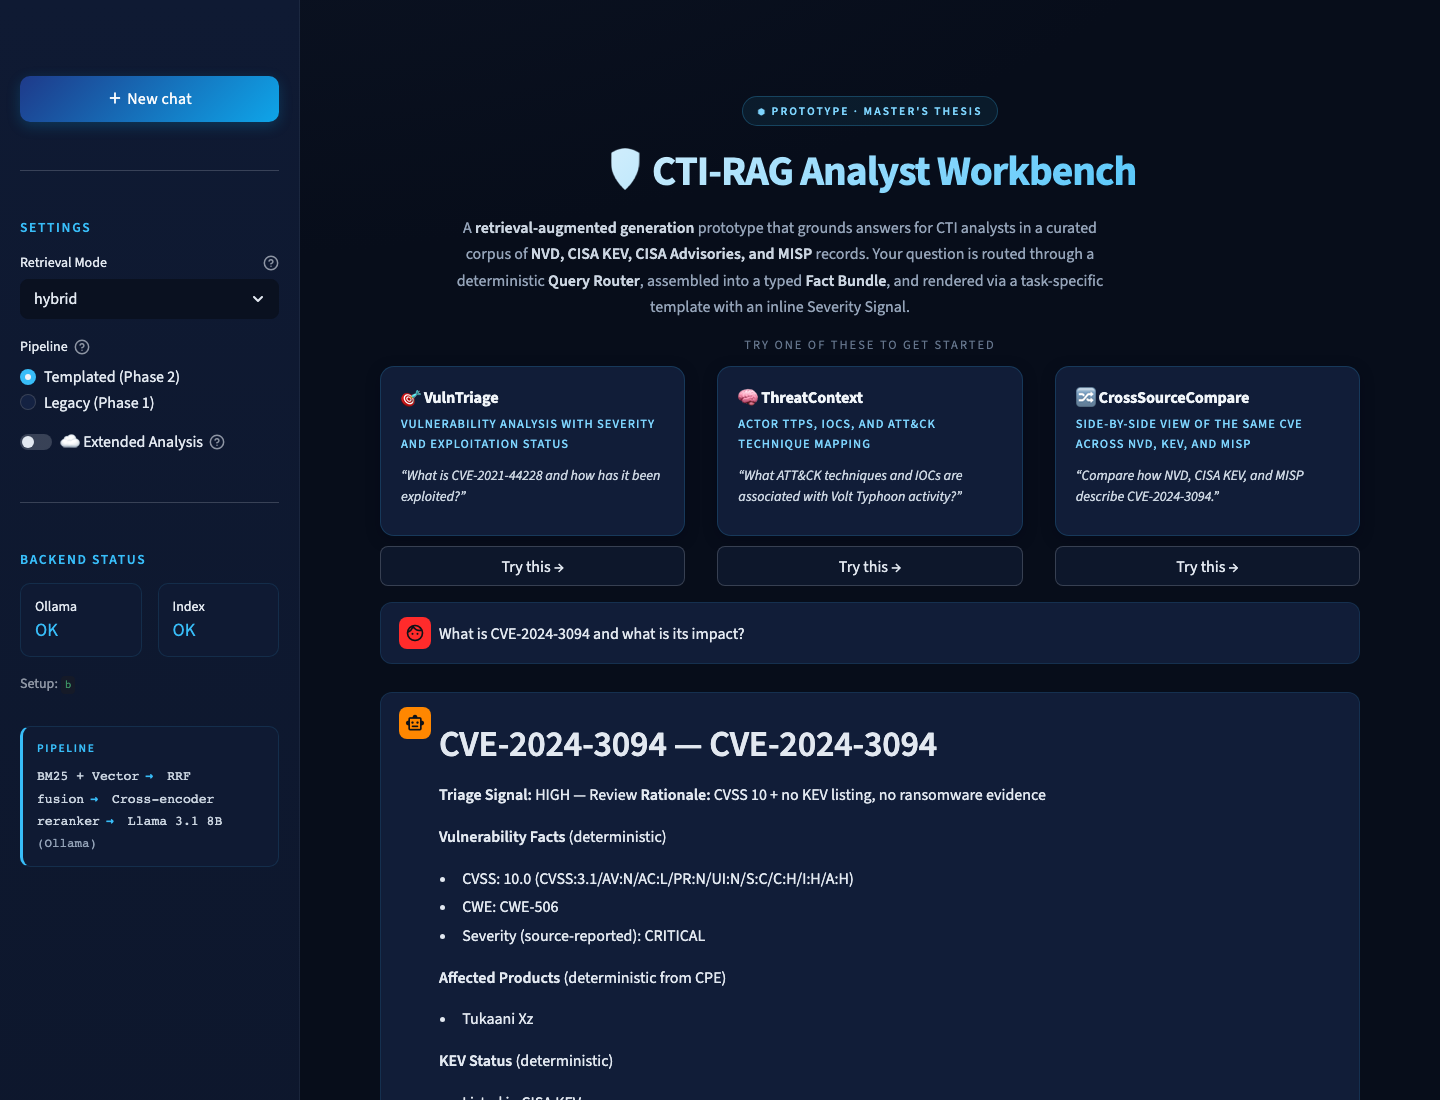
\includegraphics[width=\textwidth]{ui_chat_view}
%     \caption{Analyst-facing user interface of the prototype}
%     \label{fig:ui-overview}
% \end{figure}

\section{Evaluation design}
\label{sec:evaluation-design}
% EINZIGE Stelle fuer das Evaluationsdesign (frueheres 2.4 ist hier aufgegangen).

\subsection{Test set construction}
\label{sec:test-set}
% TODO: Query-Set (Anzahl, Kategorien, Erstellung, Ground Truth),
% Verweis auf Anhang C.
...

% TODO Tabelle: Query-Set-Uebersicht.
% \begin{table}[htbp]
%     \centering\small
%     \begin{tabular}{lrp{0.5\textwidth}}
%         \toprule
%         \textbf{Task category} & \textbf{Queries} & \textbf{Example query} \\
%         \midrule
%         Vulnerability assessment & ... & ... \\
%         IOC enrichment & ... & ... \\
%         Threat actor context & ... & ... \\
%         \bottomrule
%     \end{tabular}
%     \caption{Evaluation query set by CTI task category}
%     \label{tab:query-set}
% \end{table}

\subsection{RAGAS metrics}
\label{sec:ragas-metrics}
% TODO: verwendete Metriken definieren (faithfulness, answer relevancy,
% context precision/recall, ...), Judge-Modell, Konfiguration.
...

% TODO Tabelle: Metrik-Definitionen kompakt.
% \begin{table}[htbp]
%     \centering\small
%     \begin{tabular}{lp{0.5\textwidth}l}
%         \toprule
%         \textbf{Metric} & \textbf{Measures} & \textbf{Range} \\
%         \midrule
%         Faithfulness & ... & 0--1 \\
%         Answer relevancy & ... & 0--1 \\
%         Context precision & ... & 0--1 \\
%         Context recall & ... & 0--1 \\
%         \bottomrule
%     \end{tabular}
%     \caption{Evaluation metrics used in this thesis}
%     \label{tab:metrics}
% \end{table}

\subsection{Baseline and variant configurations}
\label{sec:baselines}
% TODO: Konfigurationsmatrix; Setup A/B dokumentieren. Kapitel 4.1
% verweist NUR hierher, keine Wiederholung dort.
...

% TODO Tabelle: Konfigurationsmatrix (wichtigste Tabelle von 3.7).
% \begin{table}[htbp]
%     \centering\small
%     \begin{tabular}{llll}
%         \toprule
%         \textbf{ID} & \textbf{Configuration} & \textbf{Retrieval} & \textbf{Generation model} \\
%         \midrule
%         V0 & Non-retrieval baseline & --- & local 8B \\
%         V1 & Sparse-only & BM25 & local 8B \\
%         V2 & Dense-only & vector & local 8B \\
%         V3 & Hybrid & BM25 + vector & local 8B \\
%         V4 & Hybrid + reranking & BM25 + vector + rerank & local 8B \\
%         V5 & Ablation: hosted model & wie V4 & hosted \\
%         \bottomrule
%     \end{tabular}
%     \caption{Baseline and variant configurations}
%     \label{tab:configurations}
% \end{table}

\subsection{Experimental protocol}
\label{sec:protocol}
% TODO: Ablauf, Reproduzierbarkeit (Seeds, Versionen, Hardware),
% Fairness-Bedingungen der Vergleiche.
...

% ======================================================================
% Kapitel 4 — Results and Critical Appraisal (Budget: ~8 Seiten)
% Enthaelt Ergebnisse UND deren Einordnung (kein separates Discussion-Kapitel):
% 4.6 Bewertung gegen Designkriterien, 4.8 Beantwortung der Forschungsfragen.
% ======================================================================
\chapter{Results and Critical Appraisal}
\label{ch:results}

\section{Experimental setup}
\label{sec:experimental-setup}
% TODO: nur konkrete Durchfuehrung (Konfigurationen, Laufumgebung, Ablauf);
% KEINE Wiederholung des Evaluationsdesigns aus \ref{sec:evaluation-design}.
% Absatz "Methodological remarks" nach Salmas Vorbild fuer Fairness-Details
% (z.B. Local-8B vs. hosted, Setup A/B).
...

% TODO Tabelle: Laufumgebung (klein); Konfigurationen NUR per Verweis
% auf Table~\ref{tab:configurations}.
% \begin{table}[htbp]
%     \centering\small
%     \begin{tabular}{ll}
%         \toprule
%         \textbf{Component} & \textbf{Version / specification} \\
%         \midrule
%         Hardware & ... \\
%         Generation model & ... \\
%         Embedding model & ... \\
%         Key software & Python ..., LangChain ..., ChromaDB ..., RAGAS ... \\
%         \bottomrule
%     \end{tabular}
%     \caption{Runtime environment of the evaluation}
%     \label{tab:environment}
% \end{table}

\section{Retrieval performance}
\label{sec:results-retrieval}
% TODO: Ergebnisse pro Retrieval-Konfiguration, Bezug zu SRQ1.
% Chart per Skript aus Eval-Daten generieren (einheitlicher Stil mit \ref{fig:generation-results}).
...

% TODO Tabelle: IR-Metriken x Konfigurationen (V1--V4 aus \ref{tab:configurations}).
% \begin{table}[htbp]
%     \centering\small
%     \begin{tabular}{lrrrr}
%         \toprule
%         \textbf{Configuration} & \textbf{P@k} & \textbf{R@k} & \textbf{MRR} & \textbf{nDCG} \\
%         \midrule
%         V1 Sparse-only & ... & ... & ... & ... \\
%         V2 Dense-only & ... & ... & ... & ... \\
%         V3 Hybrid & ... & ... & ... & ... \\
%         V4 Hybrid + rerank & ... & ... & ... & ... \\
%         \bottomrule
%     \end{tabular}
%     \caption{Retrieval performance across configurations}
%     \label{tab:retrieval-results}
% \end{table}

% TODO Abbildung: gruppiertes Balkendiagramm zu \ref{tab:retrieval-results}.
% \begin{figure}[htbp]
%     \centering
%     \includegraphics[width=\textwidth]{retrieval_results}
%     \caption{Retrieval performance by configuration and metric}
%     \label{fig:retrieval-results}
% \end{figure}

\section{Generation quality}
\label{sec:results-generation}
% TODO: RAGAS-Ergebnisse, Bezug zu SRQ1. Gleicher Chart-Stil wie 4.2.
...

% TODO Tabelle: RAGAS-Metriken x Konfigurationen (inkl. V0 Baseline!).
% \begin{table}[htbp]
%     \centering\small
%     \begin{tabular}{lrrrr}
%         \toprule
%         \textbf{Configuration} & \textbf{Faithf.} & \textbf{Ans. rel.} & \textbf{Ctx. prec.} & \textbf{Ctx. rec.} \\
%         \midrule
%         V0 Non-retrieval & ... & ... & --- & --- \\
%         V3 Hybrid & ... & ... & ... & ... \\
%         V4 Hybrid + rerank & ... & ... & ... & ... \\
%         \bottomrule
%     \end{tabular}
%     \caption{Generation quality (RAGAS) across configurations}
%     \label{tab:generation-results}
% \end{table}

% TODO Abbildung: Chart zu \ref{tab:generation-results}, Stil wie \ref{fig:retrieval-results}.
% \begin{figure}[htbp]
%     \centering
%     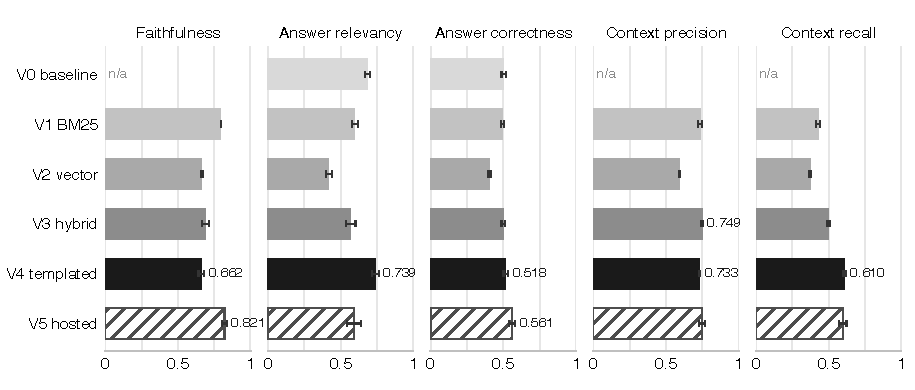
\includegraphics[width=\textwidth]{generation_results}
%     \caption{Generation quality by configuration and metric}
%     \label{fig:generation-results}
% \end{figure}

\section{Baseline comparison and ablation}
\label{sec:results-ablation}
% TODO: Vergleich gegen Baselines; Ablation (u.a. hosted Modell als
% Ablation-Zeile, Reranking an/aus). Was traegt welche Komponente bei?
...

% TODO Tabelle: wichtigste Einzeltabelle der Arbeit --- Delta gegenueber
% V0 Non-Retrieval-Baseline (beantwortet SRQ1 direkt).
% \begin{table}[htbp]
%     \centering\small
%     \begin{tabular}{lrrr}
%         \toprule
%         \textbf{Configuration} & \textbf{Metric ...} & \textbf{Metric ...} & \textbf{$\Delta$ vs. V0} \\
%         \midrule
%         V0 Non-retrieval & ... & ... & --- \\
%         V4 Hybrid + rerank & ... & ... & +... \\
%         V5 Hosted model & ... & ... & +... \\
%         \bottomrule
%     \end{tabular}
%     \caption{Ablation results relative to the non-retrieval baseline}
%     \label{tab:ablation}
% \end{table}

\section{Scenario-based evaluation of representative outputs}
\label{sec:representative-outputs}
% Qualitative Ergebnisse pro CTI-Task-Szenario (Proposal: Process Analysis).
% Pro Subsection: 1 exemplarische Antwort mit Zitaten (gekuerzt) + Bewertung
% entlang task coverage, clarity, transparency; Rest in Anhang E.
% Beleg-Basis fuer SRQ2 --- die Antwortbox in \ref{sec:rq-answers} verweist
% pro Task-Typ hierher.

\subsection{Vulnerability assessment}
\label{sec:scenario-vuln}
% TODO: CVE-/Schwachstellen-Summarization-Szenario. Dieses Szenario als
% echten UI-Screenshot zeigen (Antwort mit sichtbaren Zitaten ---
% Analog zu Salmas Audit-Trail-Screenshot); 4.5.2/4.5.3 als Text-Boxen.
...

% TODO Abbildung: UI-Screenshot Antwort mit Zitaten.
% \begin{figure}[htbp]
%     \centering
%     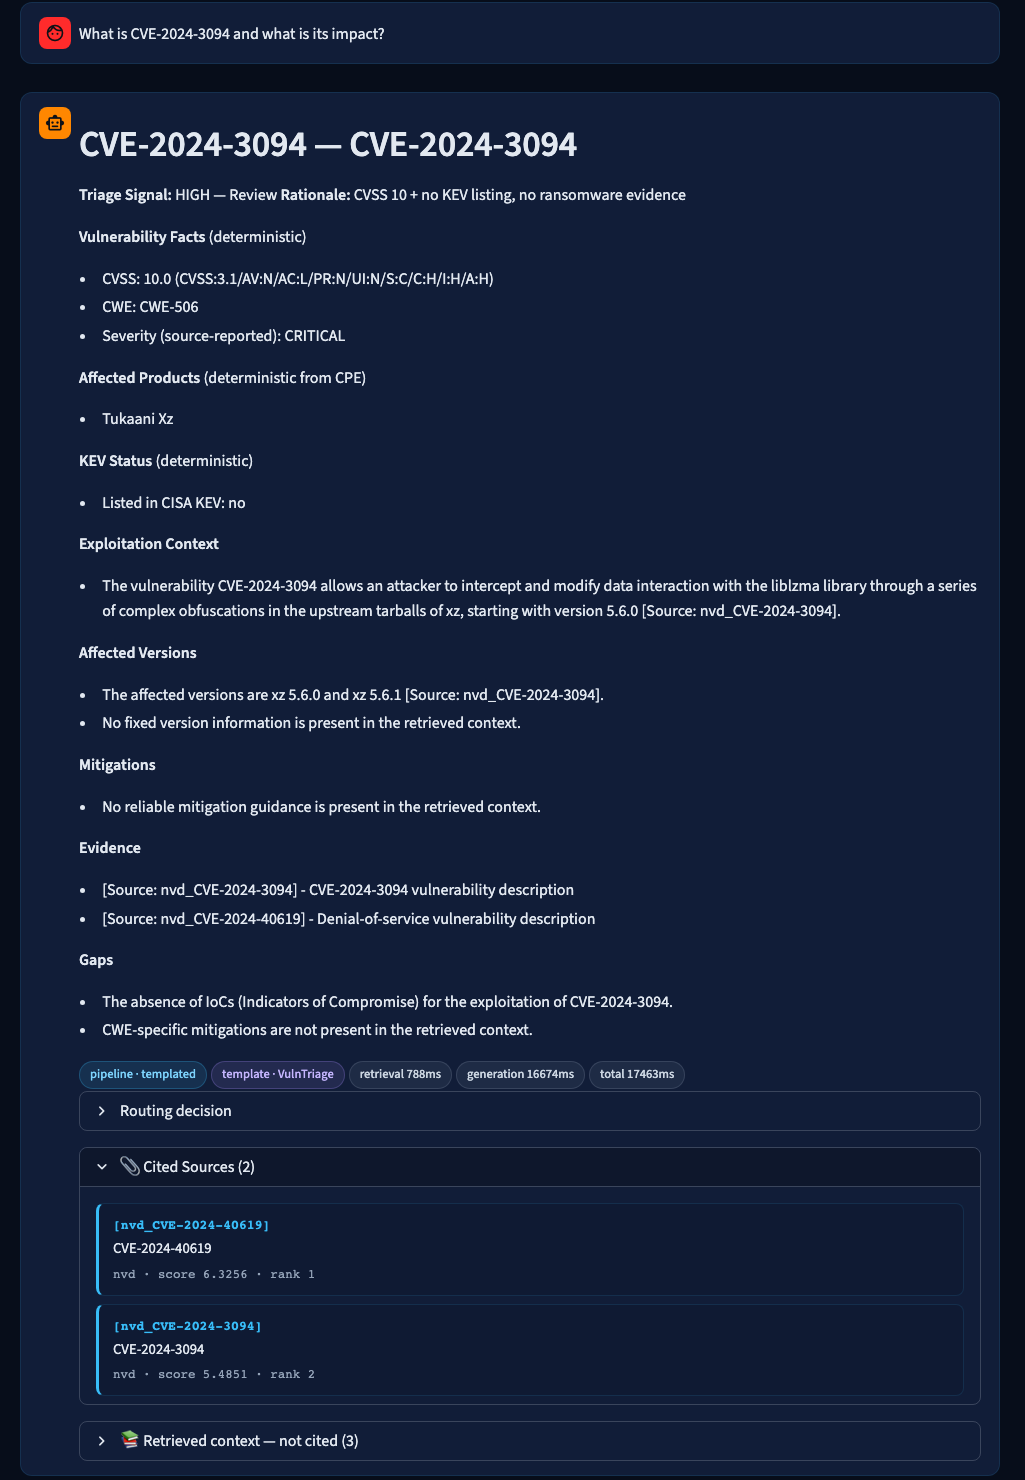
\includegraphics[width=\textwidth]{scenario_vuln_answer}
%     \caption{System response with source citations for a vulnerability
%              assessment query (excerpt)}
%     \label{fig:scenario-vuln}
% \end{figure}

\subsection{IOC enrichment}
\label{sec:scenario-ioc}
% TODO: Indicator-of-Compromise-Anreicherungs-Szenario.
% Antwortauszug als gesetzte Box (druckt sauberer als Screenshot), z.B.:
% \begin{tcolorbox}[title={Example response: IOC enrichment (excerpt)},
%                   fonttitle=\bfseries, colback=gray!4, colframe=gray!60!black,
%                   boxrule=0.5pt, arc=1mm]
% ...
% \end{tcolorbox}
...

\subsection{Threat actor context building}
\label{sec:scenario-actor}
% TODO: Threat-Actor-/TTP-Kontext-Szenario. Ebenfalls Text-Box wie 4.5.2.
...

\section{Assessment against the design criteria}
\label{sec:assessment}
% TODO: pro Kriterium C1...Cn: erfuellt / teilweise / nicht erfuellt,
% mit Verweis auf die Evidenz in 4.2--4.5 (nur referenzieren, nicht
% nacherzaehlen). Kompakte Tabelle + kurze kritische Wuerdigung.
% In der Wuerdigung den Bogen zu den Workflow-Engpaessen B1--B3
% (\ref{sec:cti}) schlagen: welcher Engpass wird durch welches erfuellte
% Kriterium adressiert (Salmas "Verbesserungen ggue. Ist-Prozess"-Effekt).
...

% TODO Tabelle: Kriterien-Assessment.
% \begin{table}[htbp]
%     \centering\small
%     \begin{tabular}{llp{0.34\textwidth}l}
%         \toprule
%         \textbf{Criterion} & \textbf{Status} & \textbf{Evidence} & \textbf{Bottleneck} \\
%         \midrule
%         C1 Evidence-linked outputs & fulfilled & Sec.~\ref{sec:representative-outputs} & B3 \\
%         C2 Hybrid retrieval & fulfilled & Tab.~\ref{tab:retrieval-results} & B1 \\
%         C3 Source integrity & partially & ... & --- \\
%         C4 Scenario-based evaluation & fulfilled & Sec.~\ref{sec:representative-outputs} & B1 \\
%         C5 Analyst-oriented presentation & ... & ... & B1 \\
%         C6 Open-source stack & fulfilled & Sec.~\ref{sec:implementation} & --- \\
%         \bottomrule
%     \end{tabular}
%     \caption{Assessment of the prototype against the design criteria}
%     \label{tab:assessment}
% \end{table}

\section{Reference model for CTI-RAG integration}
\label{sec:reference-model}
% TODO: aus den Ergebnissen verallgemeinertes Referenzmodell
% (Artefakt-Beitrag der Arbeit): Komponenten, Datenfluesse,
% Analyst-Interaktionspunkte, Governance (Proposal: Reference Modeling).
...

% TODO Abbildung: DIE Abbildung der Arbeit --- hier lohnt der meiste
% Gestaltungsaufwand. Als drawio in docs/architecture/ anlegen.
% \begin{figure}[htbp]
%     \centering
%     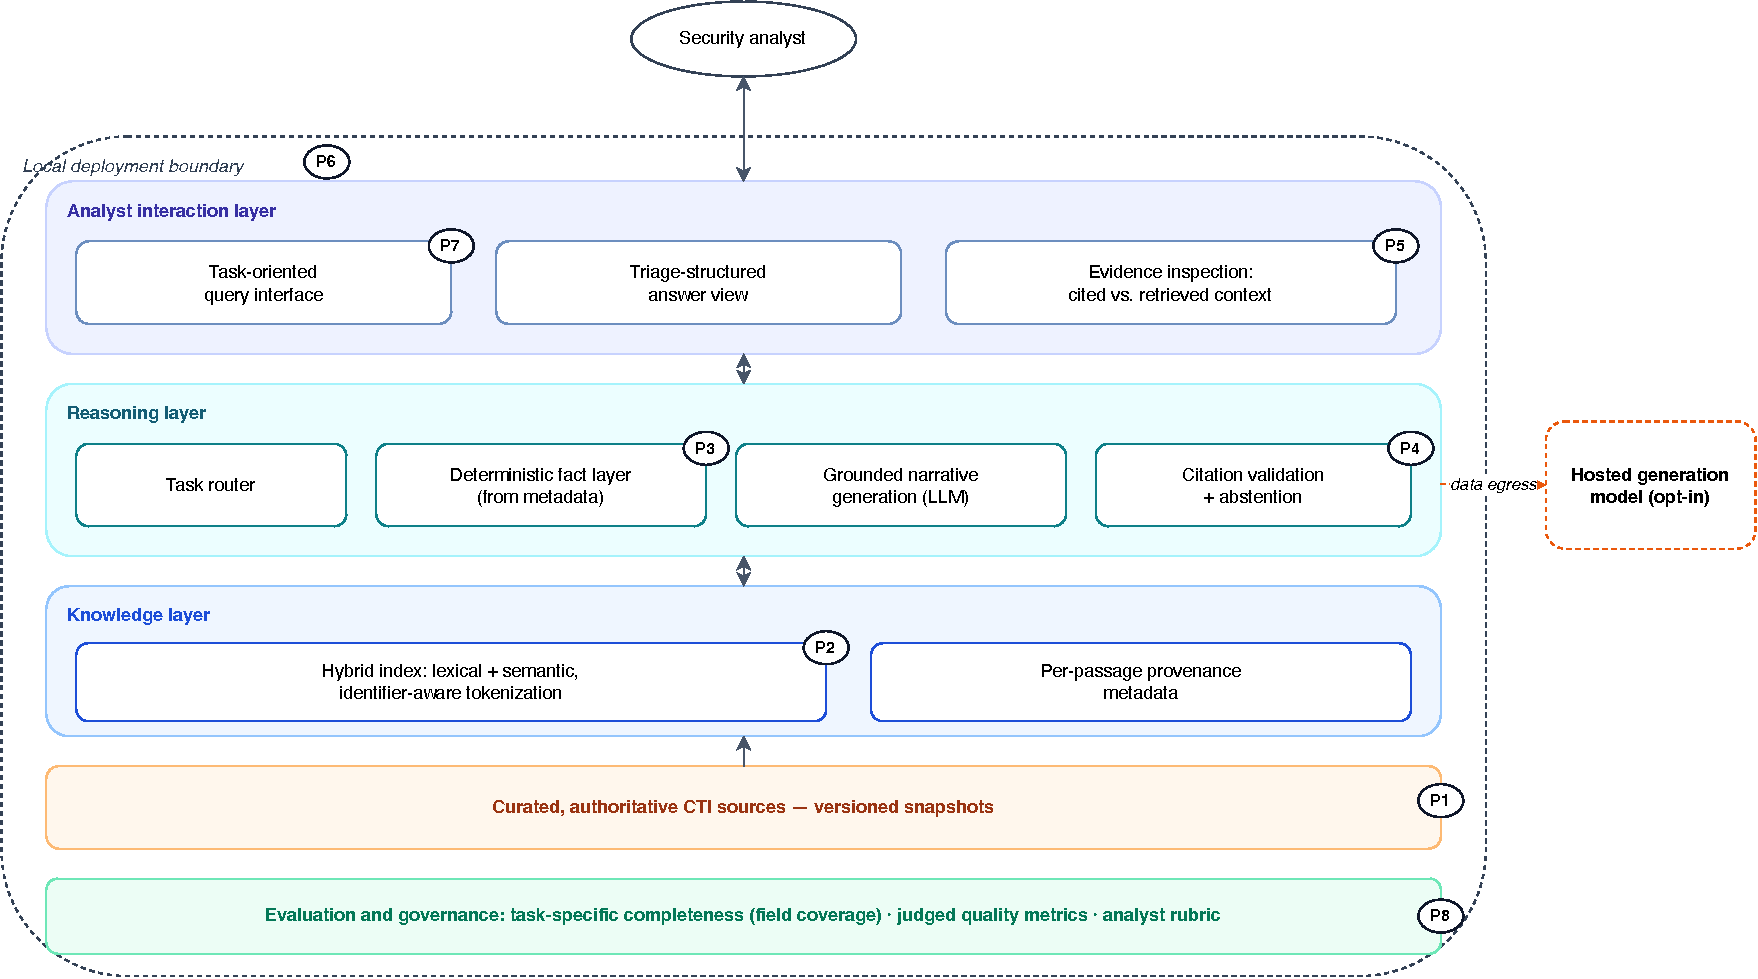
\includegraphics[width=\textwidth]{reference_model}
%     \caption{Reference model for integrating RAG-based LLM systems into
%              CTI and threat-hunting workflows}
%     \label{fig:reference-model}
% \end{figure}

\section{Answering the research questions}
\label{sec:rq-answers}
% Spiegelt die Boxen aus \ref{sec:research-questions}: Antwort in 1--2
% Saetzen + "Evidence:"-Bullets mit Verweisen auf Abschnitte/Tabellen.

\begin{rqbox}{MRQ}
    % TODO: Frage aus \ref{sec:research-questions} wiederholen, dann:
    \textbf{Answer:} ...\\[2pt]
    \textbf{Evidence:}
    \begin{itemize}
        \item ... (Section~\ref{sec:results-retrieval})
        \item ... (Section~\ref{sec:results-generation})
        \item ... (Section~\ref{sec:assessment})
    \end{itemize}
\end{rqbox}

\begin{rqbox}{SRQ1 --- Information retrieval and answer quality}
    % Beleg-Basis: RAGAS-/IR-Ergebnisse + Vergleich gegen Non-Retrieval-Baseline.
    \textbf{Answer:} ...\\[2pt]
    \textbf{Evidence:}
    \begin{itemize}
        \item ... (Section~\ref{sec:results-retrieval}, Section~\ref{sec:results-ablation})
    \end{itemize}
\end{rqbox}

\begin{rqbox}{SRQ2 --- Practical utility and workflow support}
    % Beleg-Basis: szenariobasierte qualitative Analyse, pro Task-Typ.
    \textbf{Answer:} ...\\[2pt]
    \textbf{Evidence:}
    \begin{itemize}
        \item Vulnerability assessment: ... (Section~\ref{sec:scenario-vuln})
        \item IOC enrichment: ... (Section~\ref{sec:scenario-ioc})
        \item Threat actor context: ... (Section~\ref{sec:scenario-actor})
    \end{itemize}
\end{rqbox}

\begin{rqbox}{SRQ3 --- Conceptual design}
    % Beleg-Basis: Referenzmodell/Designprinzipien aus Synthese der Ergebnisse.
    \textbf{Answer:} ...\\[2pt]
    \textbf{Evidence:}
    \begin{itemize}
        \item ... (Section~\ref{sec:reference-model}, Table~\ref{tab:design-criteria})
    \end{itemize}
\end{rqbox}

% ======================================================================
% Kapitel 5 — Conclusion, Limitations and Outlook (Budget: ~2 Seiten)
% Schlank halten: KEINE erneute Ergebnisdiskussion (die steht in Kap. 4).
% ======================================================================
\chapter{Conclusion, limitations and outlook}
\label{ch:conclusion}

\section{Summary and contributions}
\label{sec:summary}
% TODO: Was wurde gebaut und gezeigt (3--4 Absaetze); wissenschaftlicher
% und praktischer Beitrag explizit benennen (vgl. Salma 5.1).
...

\section{Limitations}
\label{sec:limitations}
% TODO: methodische Einschraenkungen als Bullets (vgl. Salma 5.2):
% Korpusgroesse/-auswahl, Query-Set-Umfang (28), LLM-as-judge-Bias
% (+ Beleg: Non-Committal-Klassifikator traf 8B UND Haiku ---
% modell-agnostische Judge-Metrik-Kritik),
% Query-Set nennt prominente CVEs -> beguenstigt parametrische Baseline
% systematisch,
% Selbstevaluierungs-Bias (szenariobasierte Bewertung durch den Autor,
% mitigiert durch das vorab definierte Raster in Anhang C),
% keine Nutzerstudie, Einzelsprache, C3 ohne Laufzeit-Credibility-Scoring,
% Context Precision/Recall sind referenzbasierte, LLM-gejudgte Proxys,
% KEINE klassischen IR-Metriken; Qrels-basierte Ranking-Evaluation bleibt
% Future Work (per-Stage-Retrieval-Traces liegen in den Artefakten vor), ...
...

\section{Future work}
\label{sec:future-work}
% TODO: zweigeteilt nach Salmas Vorbild:
% (a) praktische Roadmap (z.B. MCP-/Agent-Integration, Feed-Anbindung,
%     Multi-User-Betrieb),
% (b) wissenschaftliche Anschlussmoeglichkeiten (Nutzerstudie mit Analysten,
%     groessere Korpora, weitere Modellvergleiche, Qrels-basierte
%     IR-Evaluation auf Basis der vorhandenen Retrieval-Traces).
...

% TODO Abbildung: Roadmap-Kaskade nach Salmas Vorbild (Abb. 8 bei ihr):
% gestufte Pfeile MCP-Integration -> Feed-Anbindung -> Multi-User -> Nutzerstudie.
% \begin{figure}[htbp]
%     \centering
%     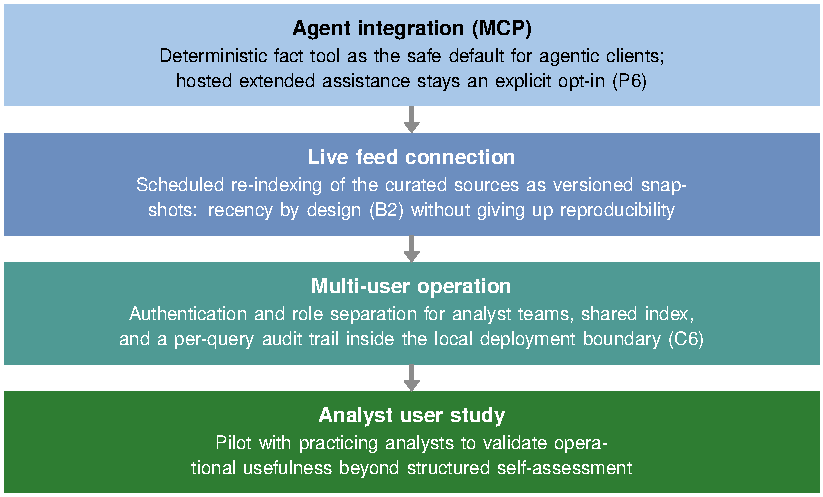
\includegraphics[width=0.85\textwidth]{roadmap_outlook}
%     \caption{Practical roadmap towards operational deployment}
%     \label{fig:roadmap}
% \end{figure}


\aitoolentry{DeepL Translate}{Translation of an article in English}{Source (XXX), Chapter X on page X-X}
\aitoolentry{Chat GPT 4.0}{Grammar and Spelling}{"Please list issues with spelling and grammar in the following text: ...", Entire document}

\clearpage
\printbibliography

\clearpage
\listoffigures

\clearpage
\listoftables

\clearpage
\listaitools

\clearpage
\addcontentsline{toc}{chapter}{\listacroname}
\chapter*{\listacroname}
\begin{acronym}[Retrieval-Augmented Generation]
    \acro{AI}{Artificial Intelligence}
    \acro{CTI}{Cyber Threat Intelligence}
    \acro{LLM}{Large Language Model}
    \acro{RAG}{Retrieval-Augmented Generation}
    \acro{MCP}{Model Context Protocol}
\end{acronym}

\clearpage
\appendix

\chapter{Prototype repository}
\label{app:repository}

The source code of the prototype is available in the following GitHub
repository:

\begin{center}
    \url{https://github.com/bhxinderj/cti-rag-analyst-support}
\end{center}

The repository contains the implementation of the prototype described in
this thesis, including configuration files, setup instructions, and
supplementary materials for reproducing the main system components. In
particular, it includes artifacts related to data ingestion and
preprocessing, retrieval and ranking, answer generation, and selected
evaluation components.

% TODO vor Abgabe: finalen Stand taggen (git tag v1.0-thesis + push).
% Falls gewuenscht, dann einen kurzen Satz zur fixierten Version wieder
% aufnehmen ("The submission refers to release tag v1.0-thesis.").

\clearpage
\chapter{Prompt templates}
\label{app:prompts}

This appendix reproduces the prompt templates of the prototype verbatim
from \texttt{src/cti\_rag/rag/prompts.py} and
\texttt{src/cti\_rag/rag/templates.py} at the evaluated state
(\texttt{evaluated-v1}). Listing~\ref{lst:full-system-prompt} is the
system prompt of the legacy mode (V1--V3),
Listing~\ref{lst:query-template} the corresponding user-message template,
Listing~\ref{lst:templated-system-prompt} the system prompt of the
templated mode (V4/V5), and Listing~\ref{lst:baseline-prompt} the prompt
of the non-retrieval baseline (V0). The per-template user messages of the
templated mode, including the pre-rendered Layer-1 blocks and target
section lists, are constructed programmatically; see the repository
(Appendix~\ref{app:repository}).

\begin{lstlisting}[caption={Legacy-mode system prompt (V1--V3), complete},
                   label={lst:full-system-prompt}]
You are a Cyber Threat Intelligence (CTI) analyst assistant. Your role
is to help security analysts by providing accurate, source-grounded
intelligence based only on the retrieved context.

Rules:
1. Use ONLY the retrieved context. Do not use prior knowledge or fill
   gaps from memory.
2. If the context is insufficient, say so explicitly and name what is
   missing.
3. Every factual statement, recommendation, or interpretation that
   comes from the context MUST end with an inline citation using the
   exact Citation Label shown for that chunk. Use the short bracket
   form: [<citation_label>]. Example:
   "Apply updates per vendor instructions [cisa_kev_CVE-2024-1709]."
   "CVE-2024-3094 is a supply-chain backdoor in xz-utils
   [nvd_CVE-2024-3094]."
4. Never invent a citation label. Only use Citation Labels that appear
   verbatim in the retrieved context.
5. Every bullet and every sentence under Summary, Why it matters,
   Recommended actions / Mitigations, and Evidence MUST end with at
   least one [<citation_label>] bracket. Lines without a bracket will
   be dropped.
6. If multiple chunks support one claim, chain their citations:
   [<label_1>] [<label_2>].
7. Do not use Markdown bold headers like **Summary:**. Use plain
   section labels exactly:
   Summary:
   Why it matters:
   Recommended actions / Mitigations:
   Evidence:
   optional: Unknowns / Gaps:
8. Use the same structure for exact CVE questions and broader CTI
   analyst questions.
9. Put at most one grounded claim per bullet or line. Do not combine
   multiple factual claims in one sentence.
10. In Recommended actions / Mitigations, include only actions
    explicitly supported by the context. If none are supported, write
    exactly: No reliable mitigation guidance is present in the
    retrieved context.
11. In Evidence, list short evidence bullets grounded in the retrieved
    context with citations.
12. Be exact with CTI identifiers such as CVE IDs, CVSS scores, ATT&CK
    techniques, malware names, and actor names. These are NOT
    citations - always add a separate [<citation_label>] bracket after
    them.
\end{lstlisting}

\begin{lstlisting}[caption={Legacy-mode user-message template},
                   label={lst:query-template}]
Based on the retrieved context above, answer the following question:

{query}

Use this response format with plain labels (no Markdown bold):
Summary:
Why it matters:
Recommended actions / Mitigations:
Evidence:
optional: Unknowns / Gaps:

Citation rules - read carefully:
- End every claim with one or more [<citation_label>] brackets from
  the retrieved context.
- Use short bracket form like [nvd_CVE-2024-3094] - not [Source: ...]
  and not [1], [2].
- Remember: ATT&CK codes like [T1059] or CVE IDs in brackets are NOT
  citations. Always add an extra [<citation_label>] after them.
- Only use Citation Labels that appear verbatim in the retrieved
  context above.
- Lines without a [<citation_label>] bracket will be discarded from
  the final answer.
\end{lstlisting}

\begin{lstlisting}[caption={Templated-mode system prompt (V4/V5), complete},
                   label={lst:templated-system-prompt}]
You are a Cyber Threat Intelligence (CTI) analyst assistant operating
in Triage Card mode.

You will receive:
1. A pre-rendered Layer-1 block that already contains deterministic
   facts (CVE-ID, CVSS, KEV status, severity signal, comparison
   tables). Do NOT repeat, re-state, or modify this block.
2. A list of retrieved context chunks with explicit citation labels.
3. A list of target sections to produce.

Rules:
1. Produce ONLY the target sections listed in the user message, in
   order.
2. Use ONLY the retrieved context. Do not use prior knowledge.
3. Every claim line MUST end with an inline citation of the form
   [Source: <citation_label>], taken verbatim from the "Allowed
   Citation Labels" list in the user message. Uncited claim lines will
   be rejected downstream and replaced with an explicit grounding
   note, so it is always better to omit a claim than to assert it
   without a citation.
4. Keep to one grounded claim per bullet or line. If a bullet would
   make two independent claims, split it into two bullets, each with
   its own [Source: ...].
5. If you cannot find support in the retrieved context for a claim you
   would otherwise make, do NOT assert it. Either omit it entirely or
   move it to the "Unknowns / Gaps" section as a statement of absence.
6. If a whole section has no support in the retrieved context, write
   exactly: "No grounded information in the retrieved context."
7. Headers, bullet scaffolding, and explicit statements of absence in
   "Unknowns / Gaps" do not require citations.
8. Be exact with CTI identifiers (CVE IDs, CVSS scores, ATT&CK
   techniques, malware names, actor names) - copy them verbatim from
   the context.
\end{lstlisting}

\begin{lstlisting}[caption={Non-retrieval baseline system prompt (V0)},
                   label={lst:baseline-prompt}]
You are a Cyber Threat Intelligence (CTI) analyst assistant. Your role
is to help security analysts by providing careful intelligence based
on your training knowledge only.

Rules:
1. Answer using your training knowledge only.
2. Do not use citations.
3. Be explicit when details are uncertain, missing, or time-sensitive.
4. Keep the response in this structure:
   Summary:
   Why it matters:
   Recommended actions / Mitigations:
   Evidence:
   Unknowns / Gaps:
5. Evidence should describe the basis of your answer without source
   citations.
6. Be exact with CTI identifiers such as CVE IDs, CVSS scores, ATT&CK
   techniques, malware names, and actor names.
\end{lstlisting}

% Hinweis: Der Baseline-User-Prompt ergaenzt die Query um eine
% Knowledge-Cutoff-Instruktion passend zum Korpus-Snapshot (2025-12-31),
% siehe build_baseline_prompt() in prompts.py und Kap. \ref{sec:generation}.


\end{document}